\chapter{Methodology}

\section{Development Approach}
\subsection*{Agile Development Techniques Applied}
The development of \textit{TRiM} followed an agile methodology (where possible, given the scope of the project), incorporating several techniques to ensure continuous progress, stakeholder alignment, and structured delivery of features throughout the project lifecycle.

A Kanban board was maintained using GitHub Projects to track the progress of all development work. Each item on the board represented a unit of work that came from a user story, and moved through columns such as \textit{Backlog}, \textit{In Progress}, and \textit{Done} as development progressed, see Figure~\ref{fig:kanban-board}. This provided a clear visual overview of the project and helped prioritise work based on immediate needs and client feedback.

\begin{figure}[H]
    \centering
    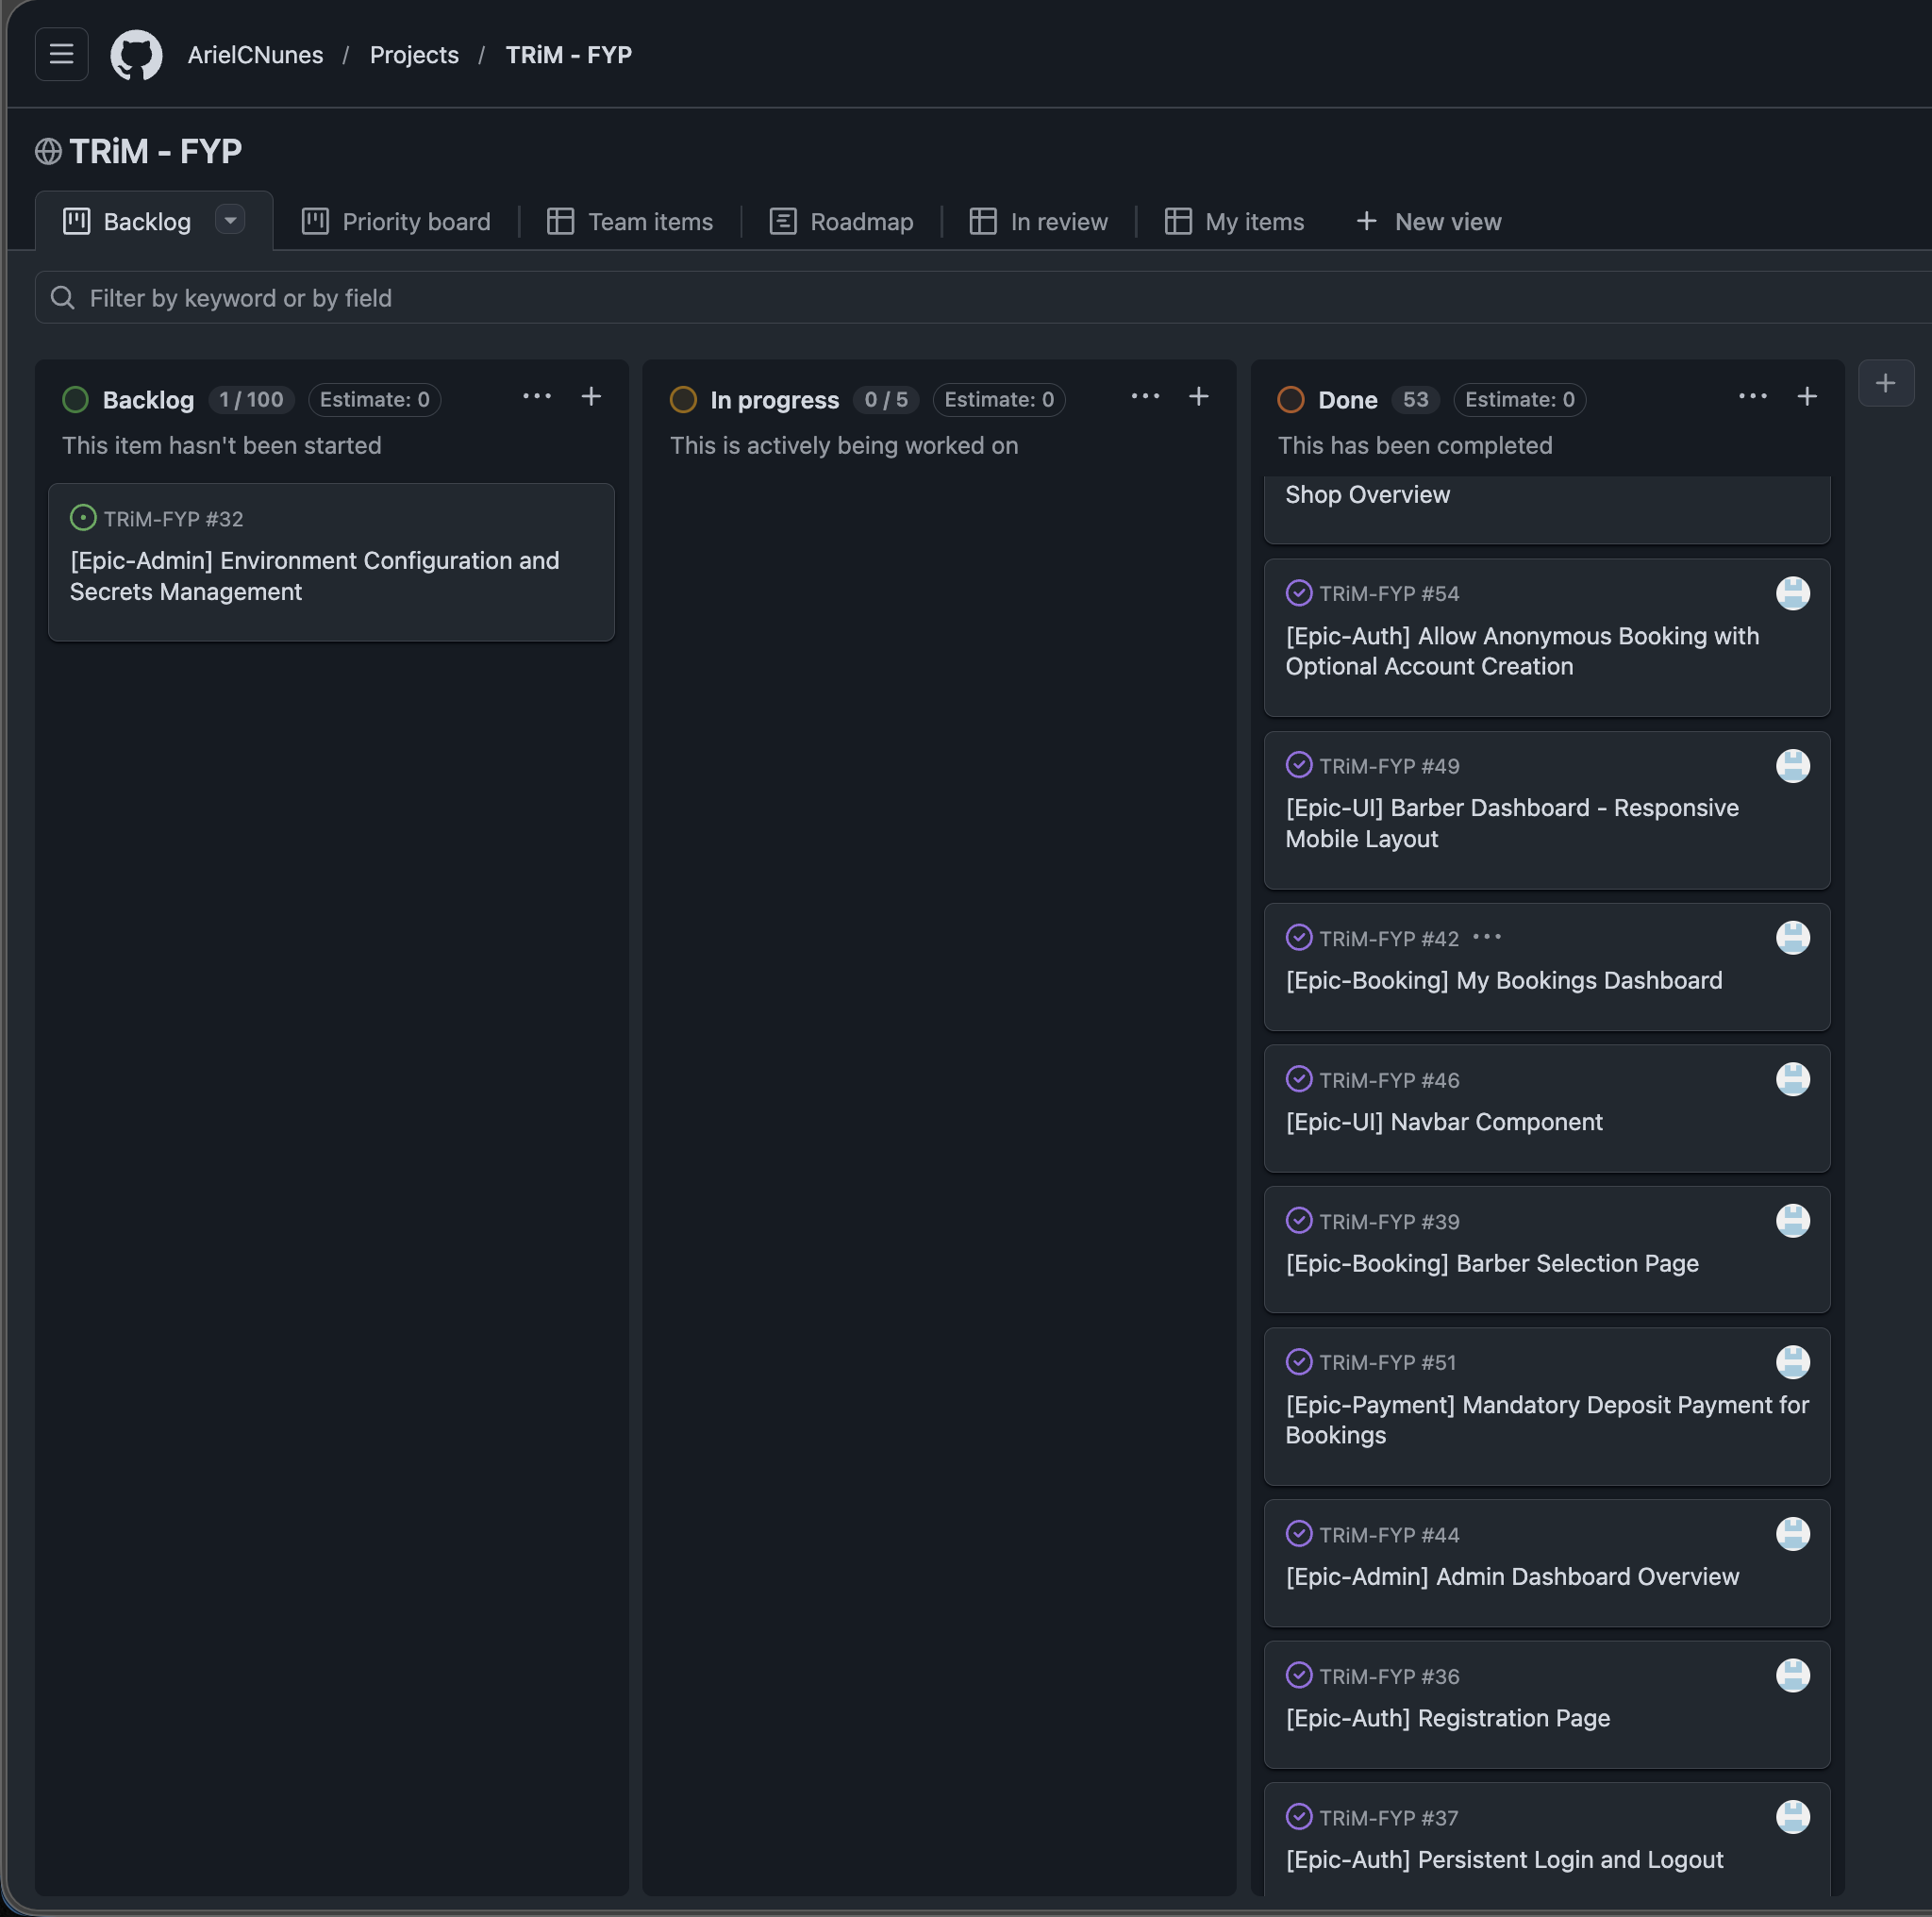
\includegraphics[width=0.7\textwidth]{images/kanbanboard.png}
    \caption{GitHub Projects Kanban board used to track development progress.}
    \label{fig:kanban-board}
\end{figure}

Requirements were captured as user stories, each documented as a GitHub Issue following a consistent structure. Every user story included four sections: a \textbf{User Story} statement written in the standard ``As a [role], I want [feature], so that [benefit]'' format; a set of \textbf{Acceptance Criteria} expressed using Given/When/Then conditions that defined the expected behaviour; a \textbf{Priority} classification (Must Have, Should Have, Could Have); and \textbf{Technical Notes} outlining relevant implementation details such as API endpoints, and UI behaviour. Figure~\ref{fig:user-story-example} illustrates a user story from the project. This format ensured that each piece of work had clearly defined scope and testable outcomes before development began.

\begin{figure}[H]
    \centering
    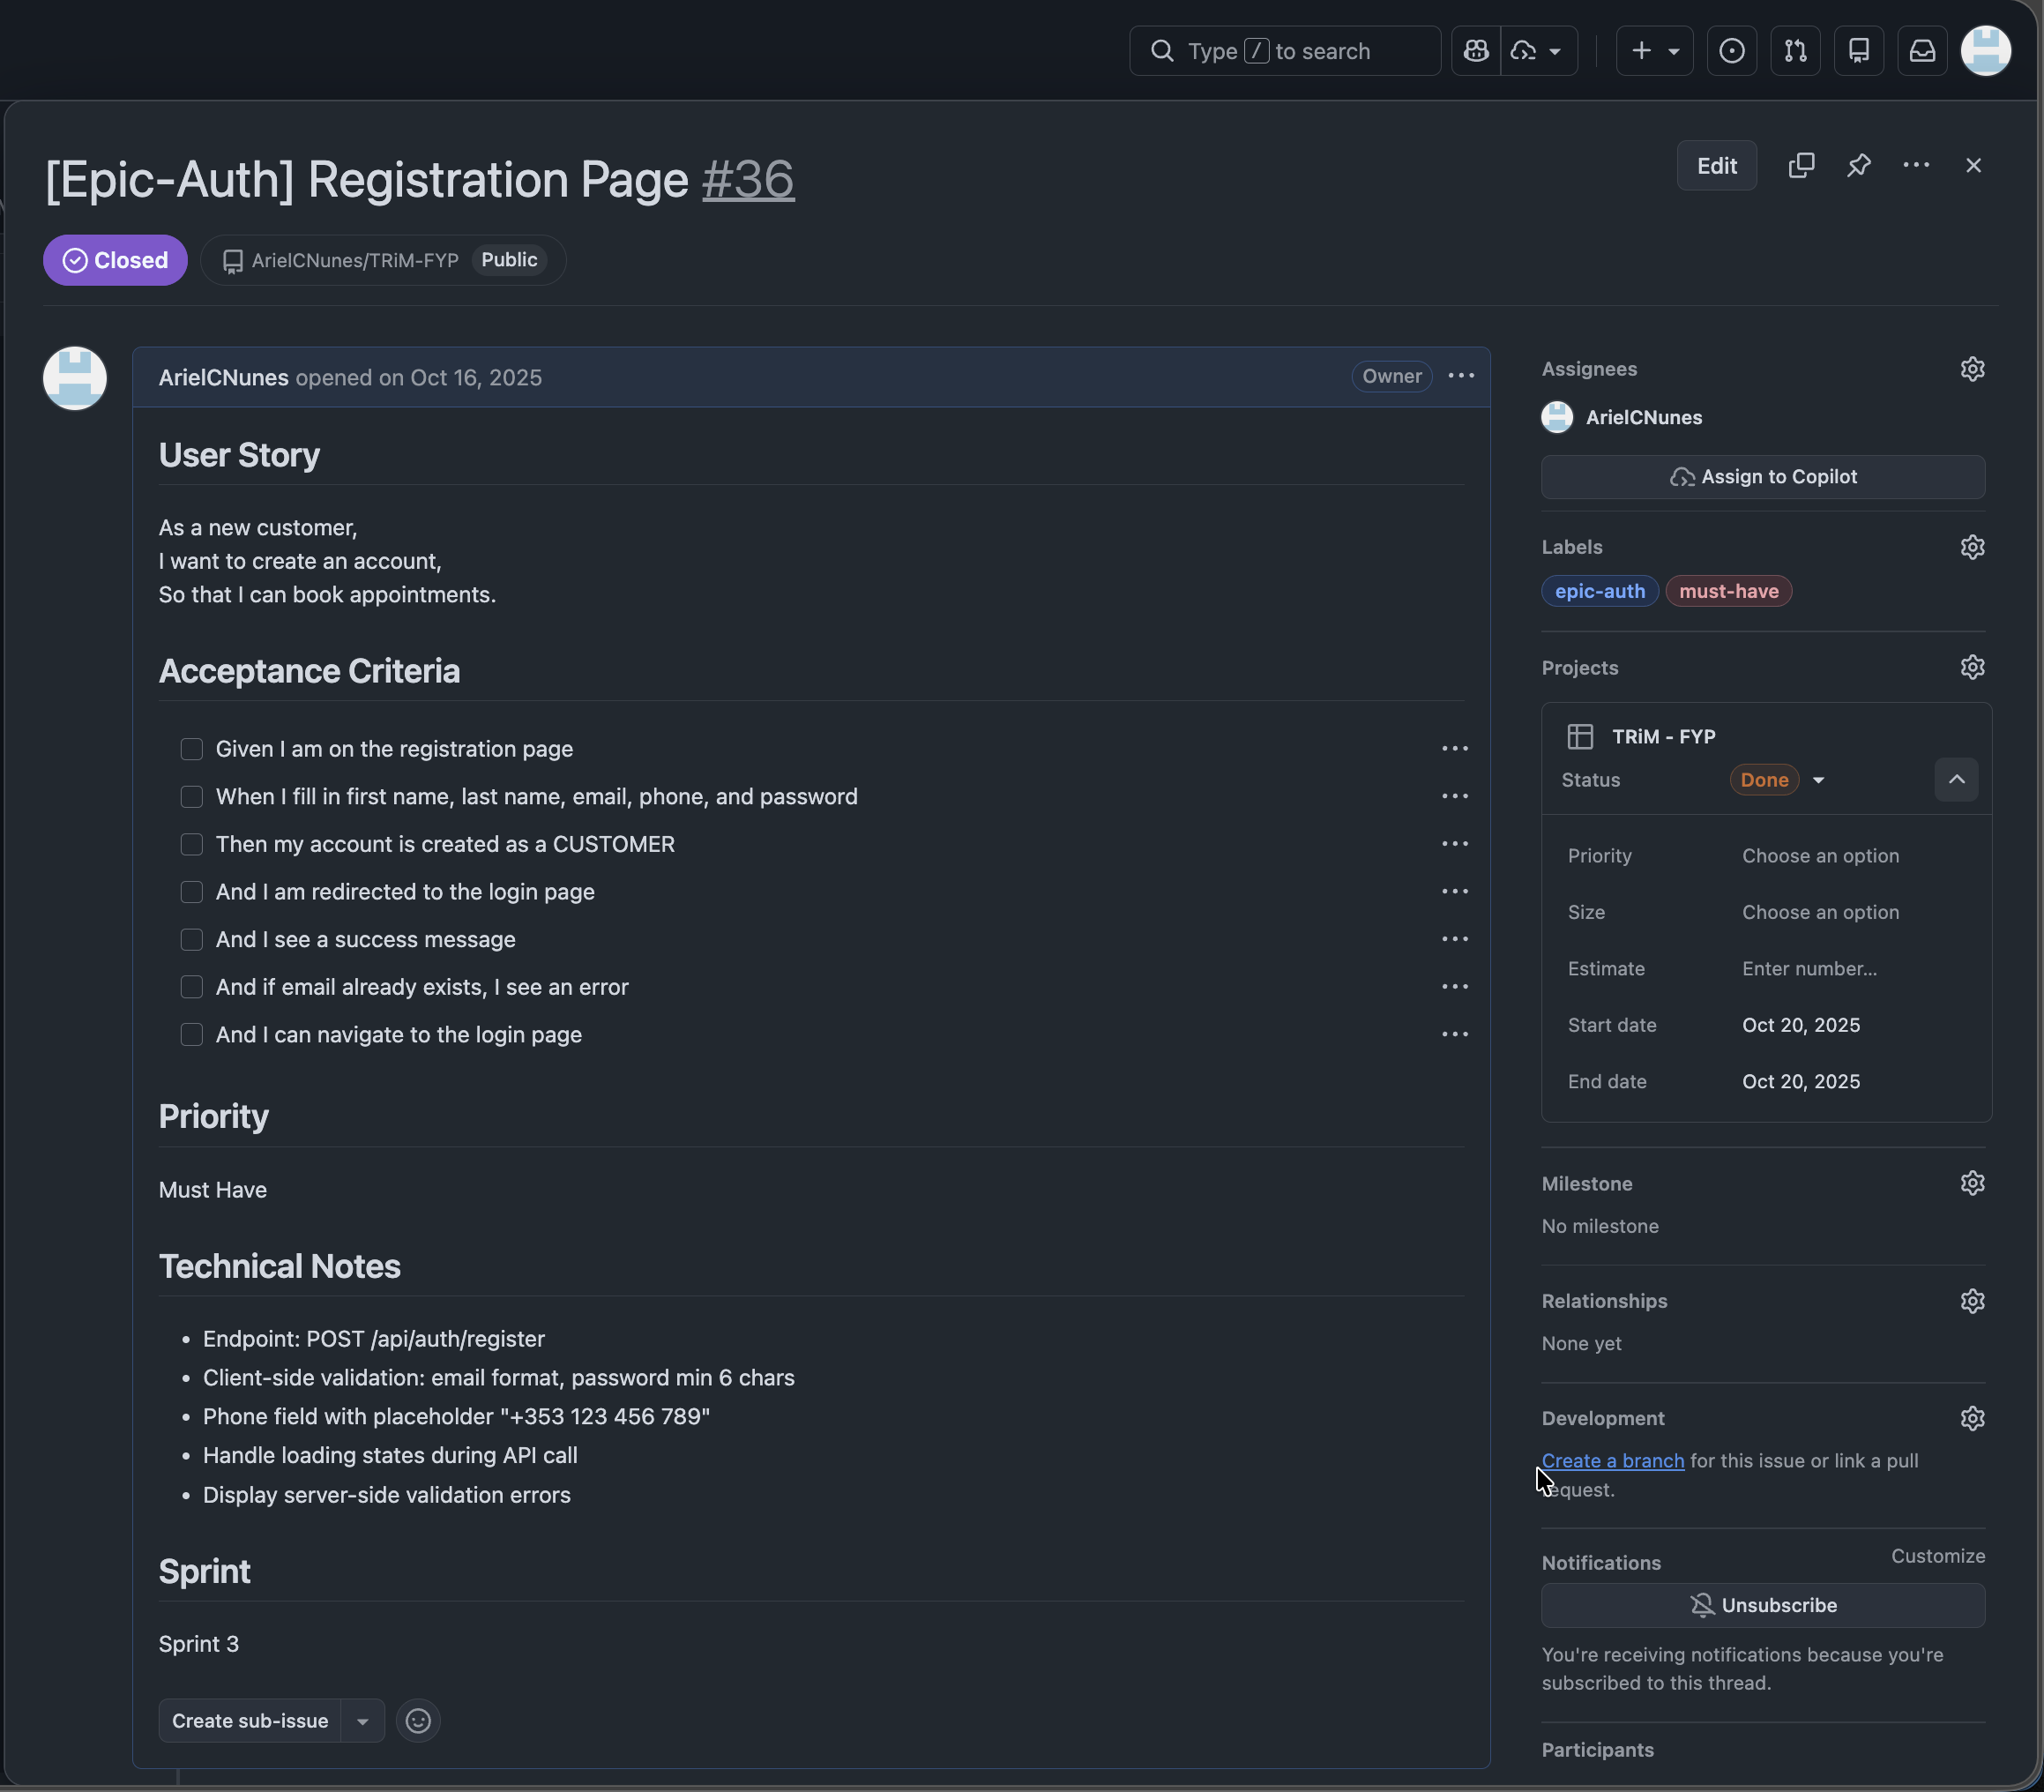
\includegraphics[width=0.7\textwidth]{images/user-story-example.png}
    \caption{Example user story with acceptance criteria, priority, and technical notes.}
    \label{fig:user-story-example}
\end{figure}

Regular communication was maintained throughout the project. Weekly meetings were held with the project supervisor to review progress, discuss technical decisions, and receive academic guidance. These meetings ensured that the project remained aligned with the FYP objectives and that research and implementation efforts were progressing. In parallel, regular meetings were conducted with the client, Jean, the owner of V7 Barbers. These meetings served as the primary mechanism for requirements gathering and validation. Early sessions focused on reviewing initial user stories and identifying additional requirements such as deposit-based payments and customer blacklisting, while later meetings involved live demonstrations of the system to get feedback on usability and functionality. This continuous feedback loop between developer, supervisor, and client ensured that \textit{TRiM} was shaped by real business needs rather than assumptions. All meetings were documented for reference.

\subsection{Version Control (GitHub)}
- InteliJ IDE + VS Code + Codespaces

\subsection{Requirements Gathering}
- Real client
- User stories

\section{Generative AI Usage}
\subsection{Code Generation with GitHub Copilot}
\subsection{Testing Automation with Claude Code}
\subsection{Code Review}

\section{Research Approach}
\subsection{Literature Search}
- Search strings and databases used
- Inclusion and exclusion criteria

\subsection{Choosing the Technology Stack}
- Reasons for selecting Java, Spring Boot, React, PostgreSQL, etc.

\section{Evaluation Methodology}
\subsection{Benchmarking With Gaitling Load Testing}
\begin{figure}[H]
    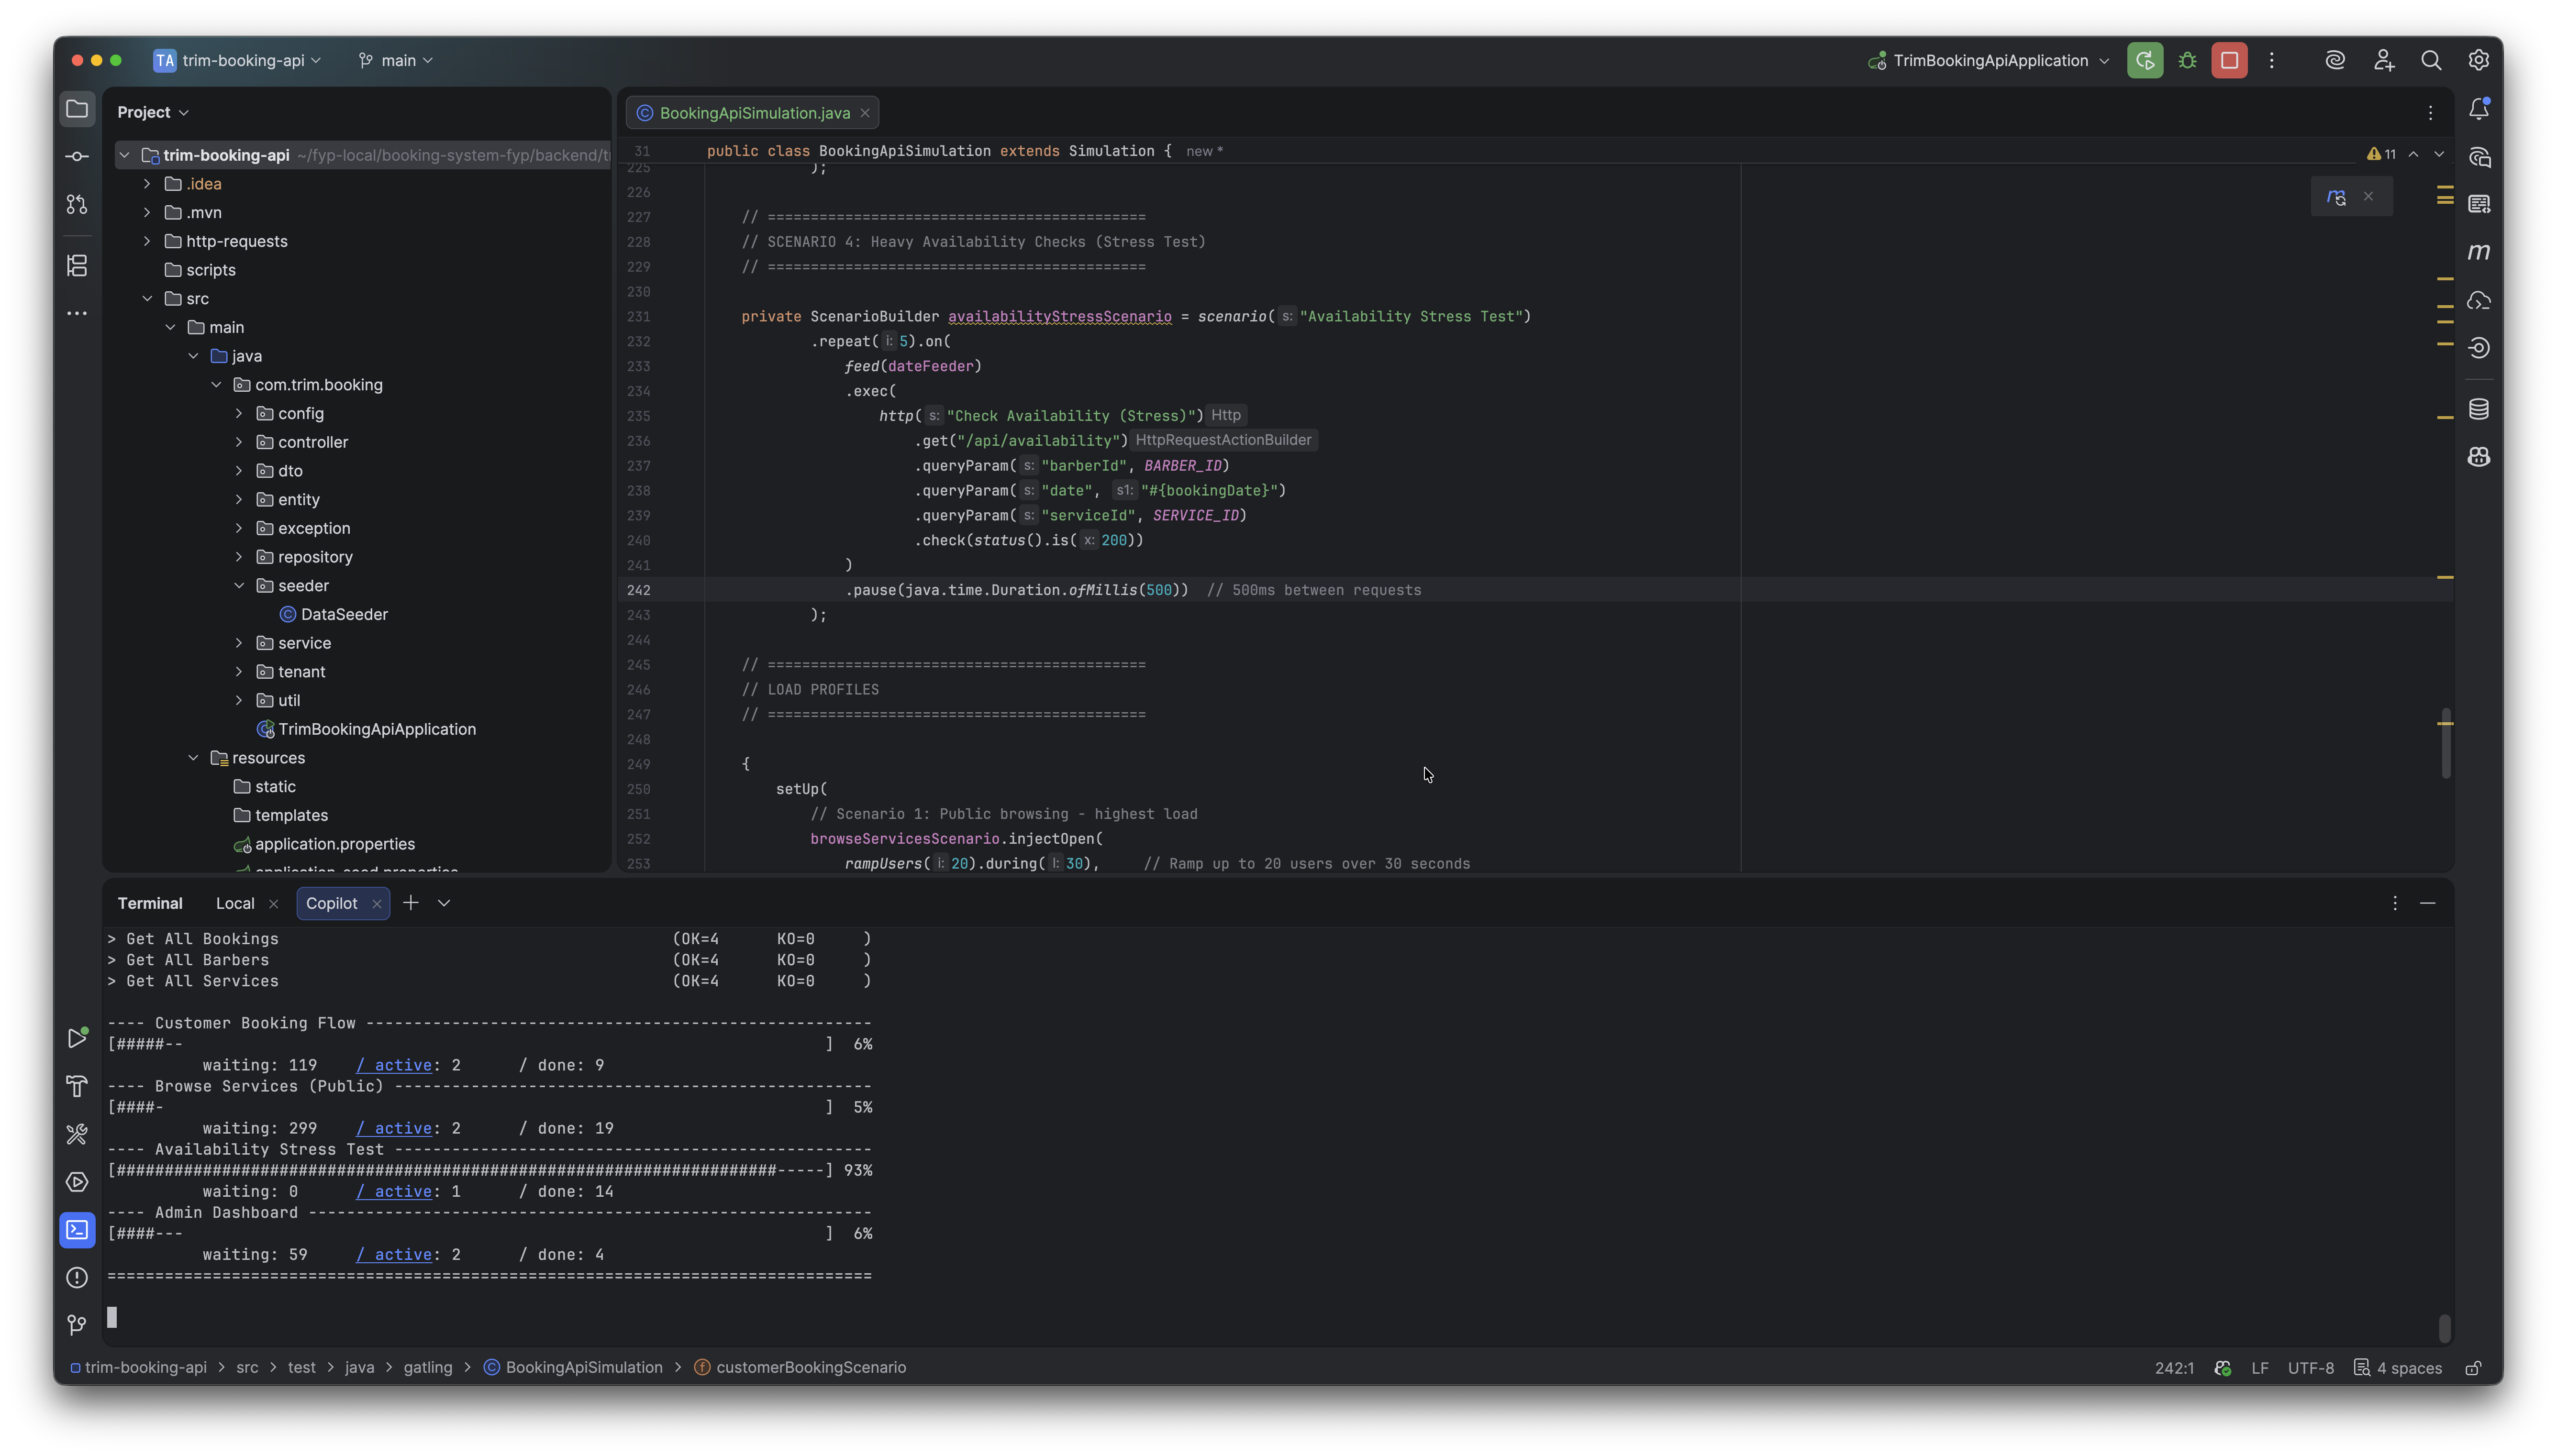
\includegraphics[width=0.9\textwidth]{images/api-benchmarking.png}
    \caption{Benchmarking API in IntelliJ IDE.}
    \label{image:apiBenchmarking}
\end{figure}

\subsection{Test Data Generation With java-seeder}
\subsection{Performance Metrics}